\PassOptionsToPackage{dvipsnames}{xcolor}
\documentclass[10pt, oneside]{article}   	% use "amsart" instead of "article" for AMSLaTeX format
\usepackage{geometry}                		% See geometry.pdf to learn the layout options. There are lots.
\geometry{letterpaper}                   		% ... or a4paper or a5paper or ... 
%\geometry{landscape}                		% Activate for rotated page geometry
%\usepackage[parfill]{parskip}    		% Activate to begin paragraphs with an empty line rather than an indent
\usepackage{graphicx}				% Use pdf, png, jpg, or eps§ with pdflatex; use eps in DVI mode
								% TeX will automatically convert eps --> pdf in pdflatex		
\usepackage{setspace}
\setstretch{0.5}

\usepackage{lmodern}
\usepackage{amsmath,amssymb,amsthm,enumitem,mathtools,xpatch}
\usepackage{bm}
\usepackage[most]{tcolorbox}
\usepackage[dvipsnames]{xcolor}
\newcommand*{\simsym}{\mathord\sim}\usepackage{amsthm}
\usepackage{float}
\usepackage{mathrsfs}
\usepackage{wrapfig, lipsum, amsthm, thmtools}
\usepackage{geometry}
 \geometry{
 a4paper,
 total={170mm,257mm},
 left=15mm,
 right = 15mm,
 top=15mm,
 bottom = 20mm
 }


\newcommand*{\Perm}[2]{{}^{#1}\!P_{#2}}%
\newcommand*{\Comb}[2]{{}^{#1}C_{#2}}%

\usepackage[framemethod=tikz]{mdframed}

\theoremstyle{definition}
\newtheorem*{exmp*}{Example}

\newtheorem*{defn}{Definition}
\surroundwithmdframed[backgroundcolor=white]{defn}

\newtheorem{cor}{Corollary}
\surroundwithmdframed[backgroundcolor=white]{cor}

\newtheorem{prop}{Proposition}
\surroundwithmdframed[backgroundcolor=white]{prop}

\newtheorem*{thm}{Theorem}
\surroundwithmdframed[backgroundcolor=white]{thm}


% tikz for probability tree

\usepackage[latin1]{inputenc}
\usepackage{tikz}
\usetikzlibrary{trees,calc,angles,positioning,intersections}

% pgfplot
\usepackage{pgfplots}
\pgfplotsset{width=10cm,compat=1.9}

% pgfplotslibrary
\usepgfplotslibrary{fillbetween}

% quotations dirty talk
\usepackage{dirtytalk}

% floor ceiling
\DeclarePairedDelimiter\ceil{\lceil}{\rceil}
\DeclarePairedDelimiter\floor{\lfloor}{\rfloor}

% diag table
\usepackage{diagbox}


\title{Introductory Probability and Statistical Applications, Second Edition \\
\large{Paul L. Meyer}}
\author{Notes and Solutions by David A. Lee}
\date{}							% Activate to display a given date or no date

\begin{document}
\maketitle
\section*{Solutions to Chapter 6: Two- and Higher-Dimensional Random Variables}


\begin{enumerate}[label=6.\arabic*]
\itemsep0em 
%Question 6.1
\item  \begin{tcolorbox}[
  colback=Cerulean!5!white,
  colframe=Cerulean!75!black]
\textbf{Suppose that the following table represents the joint probability distribution of the discrete random variable $\bm{(X,Y)}$. Evaluate all the marginal and conditional distributions.}
\end{tcolorbox}

\bgroup
\def\arraystretch{3}%  1 is the default, change whatever you need
\begin{center}
\begin{tabular}{| l | c | c | c|} 
 \hline 
  \diagbox{$Y$}{$X$} & $1$ & $2$ & $3$  \\
 \hline\hline
 $1$ & $\frac{1}{12}$ & $\frac{1}{6}$ & $0$ \\ 
 \hline
 $2$ & $0$ & $\frac{1}{9}$ & $\frac{1}{5}$ \\
 \hline
 $3$ & $\frac{1}{18}$ & $\frac{1}{4}$ & $\frac{2}{15}$ \\
 \hline
\end{tabular}
\end{center}
\egroup

\textbf{Marginal Probabilities:}

\[
\begin{aligned}
P(X = 1)  &= 1/12 + 1/18 = \boxed{5/36} \\
P(X = 2) &= 1/6 + 1/9 + 1/4 = \boxed{19/36} \\
P(X = 3) &= 1/5 + 2/15 = \boxed{1/3} \\
\end{aligned}
\qquad
\begin{aligned}
P(Y = 1) &= 1/12 + 1/6 = \boxed{1/4} \\
P(Y = 2) &= 1/9 + 1/5 = \boxed{14/45} \\
P(Y = 3) &= 1/18 + 1/4 + 2/15 = \boxed{79/180}
\end{aligned} \]

\textbf{Conditional Probabilities:}

\begin{align*}
P(X = 1 | Y = 1) &= \frac{P(X = 1, Y = 1)}{P(Y = 1)} = \frac{1/12}{3/12} = \boxed{1/3} \\
P(X = 2 | Y = 1) &= \frac{P(X = 2, Y = 1)}{P(Y = 1)} = \frac{1/6}{3/12} = \boxed{2/3} \\
P(X = 3 | Y = 1) &= \frac{P(X = 3, Y = 1)}{P(Y = 1)} = \boxed{0} \\
P(X = 1 | Y = 2) &= \frac{P(X = 1, Y = 2)}{P(Y = 2)} = \boxed{0} \\
P(X = 2 | Y = 2) &= \frac{P(X = 2, Y = 2)}{P(Y = 2)} = \frac{1/9}{14/45} = \boxed{5/14} \\
P(X = 3 | Y = 2) &= \frac{P(X = 3, Y = 2)}{P(Y = 2)} = \frac{1/5}{14/45} = \boxed{9/14} \\
P(X = 1 | Y = 3) &= \frac{P(X = 1, Y = 3)}{P(Y = 3)} = \frac{1/18}{79/180} = \boxed{10/79} \\
P(X = 2 | Y = 3) &= \frac{P(X = 2, Y = 3)}{P(Y = 3)} = \frac{1/4}{79/180} = \boxed{45/79} \\
P(X = 3 | Y = 3) &= \frac{P(X = 3, Y = 3)}{P(Y = 3)} = \frac{2/15}{79/180} = \boxed{24/79}
\end{align*}

%Question 6.2
\item  \begin{tcolorbox}[
  colback=Cerulean!5!white,
  colframe=Cerulean!75!black]
\textbf{Suppose that the two-dimensional random variable $\bm{(X,Y)}$ has joint pdf}

\[ \bm{f(x,y) = } \begin{cases} \bm{kx(x-y)}, & \bm{0 < x < 2, -x < y < x,} \\
\bm{0}, & \textbf{elsewhere}
\end{cases} \]
\end{tcolorbox}

	\begin{enumerate}
	%Question 6.2(a)
	\item  \begin{tcolorbox}[
	  colback=Cerulean!5!white,
	  colframe=Cerulean!75!black]
	\textbf{Evaluate the constant $\bm{k}$.}
	\end{tcolorbox}
	
	By assumption, $f(X, Y)$ is a joint pdf. Then we must find $k$ such that
	
	\[ \int^2_0 \int^x_{-x} kx(x-y) \ dy dx = 1 \]
	
	Proceeding, we calculate
	
	\begin{align*}
	\int^2_0 \int^x_{-x} kx^2 - kxy \ dy dx &= \int^2_0 \int^x_{-x} kx^2 - kxy \ dy dx \\
	&= \int^2_0 kx^2 y - \frac{kxy^2}{2} \Big|^x_{-x} \ dx \\
	&= \int^2_0 2kx^3 \ dx = \frac{kx^4}{2} \Big|^2_0 = 8k = 1
	\end{align*}
	
	Therefore, $\boxed{ k = 1/8 }$.
	
	%Question 6.2(b)
	\item  \begin{tcolorbox}[
	  colback=Cerulean!5!white,
	  colframe=Cerulean!75!black]
	\textbf{Find the marginal pdf of $\bm{X}$.}
	\end{tcolorbox}
	
	Integrating with respect to $y$:
	
	\begin{align*}
	\int^x_{-x} \frac{1}{8} x(x-y) \ dy = \boxed{\frac{1}{4} x^3, \quad 0 < X < 2}
	\end{align*}
	
	%Question 6.2(c)
	\item  \begin{tcolorbox}[
	  colback=Cerulean!5!white,
	  colframe=Cerulean!75!black]
	\textbf{Find the marginal pdf of $\bm{Y}$.}
	\end{tcolorbox}
	
	The bounds of $y$, in lieu of fixed numbers, are a function of $x$ itself. Combining the bounds for $x, y$, we can deduce that $0 < y < x < 2$ and $-2 < -x < y < 0$, the latter which we can rewrite as $2 > x > -y > 0$. We then must integrate $f(x,y)$ with respect to $x$ over both of these bounds.
	
	First, integrating over $(y, 2)$:
	
	\begin{align*}
	\int^2_y \frac{1}{8} x(x-y) \ dx = \boxed{\frac{1}{3} - \frac{1}{4} y + \frac{y^3}{48}, \quad 0 < y < 2}
	\end{align*}
	
	where the bound $0 < y < 2$ is apparent from the first inequality $0 < y < x < 2$; namely as $0 < x < 2$, it must be that $0 < y < 2$. Second, integrating over $(-y, 2)$:
	
	\begin{align*}
	\int^2_{-y} \frac{1}{8} x(x-y) \ dx = \boxed{\frac{1}{3} - \frac{1}{4} y + \frac{5y^3}{48}, \quad -2 < y < 0}
	\end{align*}
	
	where the bound $-2 < y < 0$ is analogously derived as in the first case, using the second inequality.
	\end{enumerate}

%Question 6.3
\item  \begin{tcolorbox}[
  colback=Cerulean!5!white,
  colframe=Cerulean!75!black]
\textbf{Suppose that the joint pdf of the two-dimensional random variable $\bm{(X,Y)}$ is given by}

\[ \bm{f(x,y) = } \begin{cases} \bm{x^2 + \frac{xy}{3},} & \bm{0 < x < 1, 0 < y < 2,} \\
\bm{0}, & \textbf{elsewhere}
\end{cases} \]

\textbf{Compute the following.}
\end{tcolorbox}

	\begin{enumerate}
	%Question 6.3(a)
	\item  \begin{tcolorbox}[
	  colback=Cerulean!5!white,
	  colframe=Cerulean!75!black]
	\textbf{$\bm{ P(X > \frac{1}{2} ) } $ }
	\end{tcolorbox}
	
	First, we must derive the marginal pdf of $X$. We do so by integrating with respect to $y$ over $(0, 2)$:
	
	\[ \int^2_0 x^2 + \frac{xy}{3} \ dy = 2x^2 + \frac{2}{3} x \]
	
	Lastly, we integrate the above result over $(1/2, 1)$:
	
	\[ \int^1_{1/2} 2x^2 + \frac{2}{3} x \ dx = \boxed{5/6} \]
	
	%Question 6.3(b)
	\item  \begin{tcolorbox}[
	  colback=Cerulean!5!white,
	  colframe=Cerulean!75!black]
	\textbf{$\bm{ P(Y < X ) } $ }
	\end{tcolorbox}
	
	There are two approaches. The direct approach is to observe that the bounds of integration for $y$ are simply $(0, x)$. If we define $A = \{ (x, y) | 0 < y < x \text{ and } 0 < x < 1 \}$, then we need only evaluate $\iint_A f(x, y) dy dx$. In the alternative, we observe that $P(Y < X) = 1 - P(Y \geq X)$, and therefore the bounds of integration for $y$ are $(x, 2)$. Defining $B = \{ (x,y) | x < y < 2 \text{ and } 0 < x < 1 \}$, the path forward then becomes $1 - \iint_B f(x,y) dy dx$. We will proceed using the first approach:
	
	\[ \int^1_0 \int^x_0 x^2 + \frac{xy}{3} \ dy dx = \boxed{ \frac{7}{24} } \]
	
	%Question 6.3(c)
	\item  \begin{tcolorbox}[
	  colback=Cerulean!5!white,
	  colframe=Cerulean!75!black]
	\textbf{$\bm{ P(Y < \frac{1}{2} | X < \frac{1}{2} ) } $ }
	\end{tcolorbox}
	
	For problems of the form $P(Y < a | X < b)$, we need only think of $f(x,y)$ as being akin to the probability of the conjunction of events $P(Y < a \cap X < b)$, and the conditional statement $P(X < b)$ represented by $\int g(x) \ dx$.
	
	The marginal density of $X$ is derived by:
	
	\[ \int^2_0 x^2 + \frac{xy}{3} \ dy = \frac{6x^2 + 2x}{3} \] 
	
	Then we calculate:
	
	\[ \frac{\int^{1/2}_0 \int^{1/2}_0 x^2 + \frac{xy}{3} \ dy dx}{\int^{1/2}_0 \frac{6x^2 + 2x}{3}} = \boxed{5/32} \]
	
	\end{enumerate}

%Question 6.4
\item  \begin{tcolorbox}[
  colback=Cerulean!5!white,
  colframe=Cerulean!75!black]
\textbf{Suppose that two cards are drawn at random from a deck of cards. Let $\bm{X}$ be the number of aces obtained and let $\bm{Y}$ be the number of queens obtained.}
\end{tcolorbox}

	\begin{enumerate}
	%Question 6.4(a)
	\item  \begin{tcolorbox}[
	  colback=Cerulean!5!white,
	  colframe=Cerulean!75!black]
	\textbf{Obtain the joint probability distribution of $\bm{(X, Y)}$.}
	\end{tcolorbox}
	
	\bgroup
\def\arraystretch{3}%  1 is the default, change whatever you need
\begin{center}
\begin{tabular}{| l | c | c | c|} 
 \hline 
  \diagbox{$Y$}{$X$} & $0$ & $1$ & $2$  \\
 \hline\hline
 $0$ & $0$ & $0$ & $\frac{4}{52} \cdot \frac{3}{51} = \frac{1}{221}$ \\ 
 \hline
 $1$ & $0$ & $\frac{4}{52} \cdot \frac{4}{51} = \frac{4}{663}$ & $0$ \\
 \hline
 $2$ & $\frac{4}{52} \cdot \frac{3}{51} = \frac{1}{221}$ & $0$ & $0$ \\
 \hline
\end{tabular}
\end{center}
\egroup
	
	%Question 6.4(b)
	\item  \begin{tcolorbox}[
	  colback=Cerulean!5!white,
	  colframe=Cerulean!75!black]
	\textbf{Obtain the marginal distribution of $\bm{X}$ and of $\bm{Y}$.}
	\end{tcolorbox}
	
	\[
	\begin{aligned}
	P(X = 0) &= \boxed{\frac{1}{221}} \\
	P(X = 1) &= \boxed{\frac{4}{663}} \\
	P(X = 2) &= \boxed{\frac{1}{221}} \\
	\end{aligned}
	\qquad
	\begin{aligned}
	P(Y = 0) &= \boxed{\frac{1}{221}} \\
	P(Y = 1) &= \boxed{\frac{4}{663}} \\
	P(Y = 2) &= \boxed{\frac{1}{221}}
	\end{aligned} \]
	
	%Question 6.4(c)
	\item  \begin{tcolorbox}[
	  colback=Cerulean!5!white,
	  colframe=Cerulean!75!black]
	\textbf{Obtain the conditional distribution of $\bm{X}$ (given $\bm{Y}$) and of $\bm{Y}$ (given $\bm{X}$).}
	\end{tcolorbox}
	
	\[
	\begin{aligned}
	P(X = 0 | Y = 2) &= \frac{P(X = 0, Y = 2)}{P(Y = 2)} = \boxed{1} \\
	P(X = 1 | Y = 1) &= \frac{P(X = 1, Y = 1)}{P(Y = 1)} = \boxed{1} \\
	P(X = 2 | Y = 0) &= \frac{P(X = 2, Y = 0)}{P(Y = 2)} = \boxed{1} \\
	\end{aligned}
	\qquad
	\begin{aligned}
	P(Y = 0 | X = 2) &= \frac{P(Y = 0, X = 2)}{P(X = 2)} = \boxed{1} \\
	P(Y = 1 | X = 1) &= \frac{P(Y = 1, X = 1)}{P(X = 1)} = \boxed{1} \\
	P(Y = 2 | X = 0) &= \frac{P(Y = 2, X = 0)}{P(X = 0)} = \boxed{1}
	\end{aligned} \]
	
	\end{enumerate}

%Question 6.5
\item  \begin{tcolorbox}[
  colback=Cerulean!5!white,
  colframe=Cerulean!75!black]
\textbf{For what value of $\bm{k}$ is $\bm{f(x,y) = ke^{-(x+y)}}$ a joint pdf of $\bm{(X,Y)}$ over the region $\bm{0 < x < 1, 0 < y < 1}$?}
\end{tcolorbox}

We must find the value of $k$ such that

\[ \int^1_0 \int^1_0 ke^{-x} e^{-y} \ dy dx = 1 \]

Evaluating the integral and isolating $k$ yields $\boxed{k = \frac{1}{(1 - e^{-1})^2}}$.

%Question 6.6
\item  \begin{tcolorbox}[
  colback=Cerulean!5!white,
  colframe=Cerulean!75!black]
\textbf{Suppose that the continuous two-dimensional random variable $\bm{(X,Y)}$ is uniformly distributed over the square whose vertices are $\bm{(1,0), (0,1), (-1,0),}$ and $\bm{(0,-1)}$. Find the marginal pdf's of $\bm{X}$ and of $\bm{Y}$.}
\end{tcolorbox}


	\begin{center}
	\begin{tikzpicture}[scale=0.75]
	\begin{axis}[
    		axis lines = center,
		xmax=1.5,
		xmin=-1.5,
		ymax=1.5,
		ymin=-1.5,
   		 xlabel = \(  \),
   		 ylabel = {\( \)},
		 xtick={-1,0,1},
    		 xticklabels={$-1$,$0$,$1$},
		 ytick={-1,0,1},
		 yticklabels={$-1$,$0$,$1$},
		]
	\addplot[samples=500,domain=0:1, color=red, style=thick]{-x + 1} node[above = 25 pt] (a) {$y = -x + 1$};
	\addplot[samples=500,domain=0:1, color=red, style=thick]{x - 1} node[below = 25 pt] (b) {$y = x - 1$};
	\addplot[samples=500,domain=-1:0, color=red, style=thick]{x + 1} node[left=110pt of a] {$y = x + 1$};
	\addplot[samples=500,domain=-1:0, color=red, style=thick]{-x - 1} (-1,0) node[left=110pt of b] {$y = -x - 1$};
	\end{axis}
	\end{tikzpicture}
	\quad
	\begin{tikzpicture}[scale=0.75]
	\begin{axis}[
    		axis lines = center,
		xmax=1.5,
		xmin=-1.5,
		ymax=1.5,
		ymin=-1.5,
   		 xlabel = \(  \),
   		 ylabel = {\( \)},
		 xtick={-1,0,1},
    		 xticklabels={$-1$,$0$,$1$},
		 ytick={-1,0,1},
		 yticklabels={$-1$,$0$,$1$},
		]
	\addplot[samples=500,domain=0:1, color=red, style=thick]{-x + 1} node[above = 25 pt] (a) {$x = -y + 1$};
	\addplot[samples=500,domain=0:1, color=red, style=thick]{x - 1} node[below = 25 pt] (b) {$x = y - 1$};
	\addplot[samples=500,domain=-1:0, color=red, style=thick]{x + 1} node[left=110pt of a] {$x = y - 1$};
	\addplot[samples=500,domain=-1:0, color=red, style=thick]{-x - 1} (-1,0) node[left=110pt of b] {$x = -y - 1$};
	\end{axis}
	\end{tikzpicture}
	\end{center}

	Since we are dealing with a uniform joint distribution, we know that $f(x,y) = 1 / \text{area}(R)$, where $R$ is the region over which $(X,Y)$ is distributed. The region defined above is a square with length $\sqrt{2}$, so $\boxed{f(x,y) = 1/2}$.
	
	To find the marginal pdf of $X$, we calculate piecewise over the intervals $(0, 1)$ and $(-1, 0)$:
	
	\begin{align*}
	g(x) &= \begin{dcases}
	 \int^{-x + 1}_{x - 1} \frac{1}{2} \ dy, \quad 0 < x < 1 \\
	 \int^{x+1}_{-x-1} \frac{1}{2} \ dy, \quad -1 < x < 0
	 \end{dcases} \\
	 &= \begin{dcases}
	 1 - x, \quad 0 < x < 1 \\
	 1 + x, \quad -1 < x < 0
	 \end{dcases}
	 \end{align*}

	In the interest of brevity, we may write $\boxed{g(x) = 1 - |x|, -1 < x < 1}$ is the marginal pdf of $X$. By symmetry, $\boxed{h(y) = 1 - |y|, -1 < y < 1}$ is the marginal pdf of $Y$.

%Question 6.7
\item  \begin{tcolorbox}[
  colback=Cerulean!5!white,
  colframe=Cerulean!75!black]
\textbf{Suppose that the dimensions, $\bm{X}$ and $\bm{Y}$, of a rectangular metal plate may be considered to be independent continuous random variables with the following pdfs.}

\[
\bm{X: g(x) =} \begin{dcases}
\bm{x - 1}, \quad \bm{1 < x \leq 2} \\
\bm{-x + 3} \quad \bm{2 < x < 3} \\
\bm{0}, \quad \textbf{elsewhere}
\end{dcases}
\]
\[
\bm{Y: h(y) =} \begin{dcases}
\bm{\frac{1}{2}}, \quad \bm{2 < y < 4} \\
\bm{0}, \quad \textbf{elsewhere}
\end{dcases}
\]

\textbf{Find the pdf of the area of the plate, $\bm{A = XY}$.}
\end{tcolorbox}

Combining the bounds for $X$ and $Y$, we can derive the following bounds for $x$ in terms of the area $a$:

\begin{align*}
&1 < x \leq 2 \quad \text{and} \quad 2 < y < 4 \\
\implies &2 < \frac{a}{x} < 4 \\
\implies &\boxed{1 < x < \frac{a}{2}} \quad \text{and} \quad \boxed{\frac{a}{4} < x \leq 2} \\
&2 < x < 3 \quad \text{and} \quad 2 < y < 4 \\
\implies &2 < \frac{a}{x} < 4 \\
\implies &\boxed{ 2 < x < \frac{a}{2} } \quad \text{and} \quad \boxed{ \frac{a}{4} < x < 3 }
\end{align*}

In general, derivation of the pdf of a product of two random variables $X, Y$ with corresponding pdfs $g(x), h(y)$ is given by

\[ p(w) = \int^{+\infty}_{-\infty} g(u) h \Big( \frac{w}{u} \Big) \Big| \text{det} (\bm{J}) \Big| \ du \]

where $w = xy$ and $x = u$, and $\text{det}(\bm{J})$ is the Jacobian determinant of $x, y$ in terms of $u, w$.\footnote{For some simple, geometric intuition behind the Jacobian term, check out this Cross Validated post. No measure theory or any advanced understanding needed beyond the volume of a 3-dimensional parallelogram. https://math.stackexchange.com/questions/267267/intuitive-proof-of-multivariable-changing-of-variables-formula-jacobian-withou} Here, $a = xy$ and $x = u$, implying $x = u$ and $y = a/x$. we derive the Jacobian as:

\begingroup
\renewcommand*{\arraystretch}{3.5}
\[ J = \begin{vmatrix}
\frac{\partial x}{\partial a} & \frac{\partial x}{\partial u} \\
\frac{\partial y}{\partial a} & \frac{\partial y}{\partial u}
\end{vmatrix} = \begin{vmatrix}
0 & 1 \\
\frac{1}{u} & -\frac{a}{u^2}
\end{vmatrix} = -\frac{1}{u}
 \]
 \endgroup

Therefore, we proceed by deriving the pdfs of the joint distribution at each of the previously derived intervals:

\begin{align*}
p(a) = \int^{a/2}_1 g(u) h \Big( \frac{a}{u} \Big) \frac{1}{u} \ du &= \int^{a/2}_1 (x-1) \Big( \frac{1}{2} \Big) \frac{1}{x} \ dx \\
&= \boxed{ \frac{a-2}{4} - \frac{1}{2} \ln \frac{a}{2}, \quad 2 < a \leq 4 } \\
p(a) = \int^2_{a/4} g(u) h \Big( \frac{a}{u} \Big) \frac{1}{u} \ du &= \int^2_{a/4} (x-1) \Big( \frac{1}{2} \Big) \frac{1}{x} \ dx \\
&= \boxed{ \frac{8-a}{8} + \frac{1}{2} \ln \frac{a}{8}, \quad 4 < a \leq 8 } \\
p(a) = \int^{a/2}_2 g(u) h \Big( \frac{a}{u} \Big) \frac{1}{u} \ du &=  \int^{a/2}_2 (-x + 3) \Big( \frac{1}{2} \Big) \frac{1}{x} \ dx \\
&= \boxed{ \frac{4-a}{4} + \frac{3}{2} \ln \frac{a}{4}, \quad 4 < a < 6 } \\
p(a) = \int^3_{a/4} g(u) h \Big( \frac{a}{u} \Big) \frac{1}{u} \ du &= \int^3_{a/4} (-x + 3) \Big( \frac{1}{2} \Big) \frac{1}{x} \ dx \\
&= \boxed{ \frac{a-12}{8} + \frac{3}{2} \ln \frac{12}{a}, \quad 8 < a < 12 }
\end{align*}

In order to derive the bounds for $a$, we simply determine which values of $a$ satisfy the following:

\begin{align*}
\frac{a}{2} &\in (1, 2] \implies 2 < a \leq 4 \\
\frac{a}{4} &\in (1, 2] \implies 4 < a \leq 8 \\
\frac{a}{2} &\in (2,3) \implies 4 < a < 6 \\
\frac{a}{4} &\in (2,3) \implies 8 < a < 12
\end{align*}

All these statements are saying is the either the lower or upper bound that is a function of $a$ must ultimately lie within the interval of $x$ for which $f(x)$ is nonzero.

Taking a step back, each of the piecewise densities derived above give us the probability of the area $a$ lying within some range $\alpha$ to $\beta$. \textbf{A subtle but critical point is as follows: there are mutually exclusive events leading to the outcome that $\bm{a \in (\alpha,\beta)}$.} For instance, we may have $x \in (1,2]$ or -- namely, mutually exclusive or -- $x \in (2,3)$ with $y \in (2,4)$ and come to the outcome $a \in (4,6)$. The individual densities we derived from each case, as in the case of probabilities of mutually exclusive events, must be summed to get the ``total contribution" of the probabilities of all disjoint events leading to the same outcome. 

This explanation makes the most sense when thinking of it geometrically. In more precise terms, the \textit{area} under the density derived from one of the events is the probability of that event leading to an outcome. The areas of the densities for all other disjoint events leading \textit{to that same outcome} must then be summed to get the \textit{total} contribution of probabilities of events leading to that outcome.

Now, in the first two piecewise densities, we have $1 < x \leq 2$ and $2 < y < 4$, implying $2 < a < 8$. The union intervals of $a$ for which these two piecewise densities are defined indeed spans the entirety of $2 < a < 8$. However, in the latter two piecewise densities, we have $2 < x < 3$ and $2 < y < 4$ which implies $4 < a < 12$. Particularly, $(4, 6) \cup (8, 12)$ implies a gap; namely $[6,8]$ is unaccounted for. Conceptually, we have ``missing events" that need to lead to the outcome $a \in (6,8)$. 

To further investigate this point, consider the following contour plot of the area of the plate $a = xy$ over the bounds of $x$ and $y$ for which their respective pdfs are non-zero: \footnote{Thank you to whuber on Cross Validated for the tip here. See: https://stats.stackexchange.com/questions/609878/2-dimensional-functions-of-random-variables-with-piecewise-densities}

	\begin{center}
	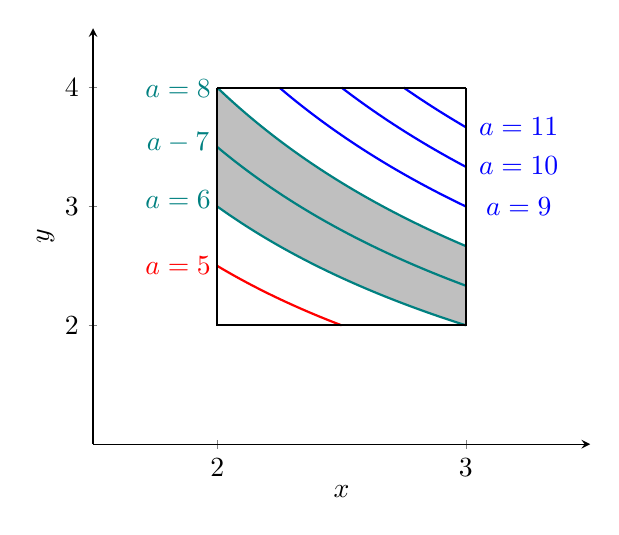
\begin{tikzpicture}[scale=0.75]
	\begin{axis}[
    		axis lines = left,
		xmax=3.5,
		xmin=1.5,
		ymax=4.5,
		ymin=1,
   		 xlabel = \( x \),
   		 ylabel = {\( y \)},
		 xtick={2,3},
    		 xticklabels={$2$,$3$},
		 ytick={2,3,4},
		 yticklabels={$2$,$3$,$4$},
		]
		 \node (some node) at (100,150) (a) {};
		  \node (some node) at (150,200) (c) {};
	\addplot[samples=500,domain=2:2.5, color=red, style=thick]{5/x} node[left = 40 pt of a] (b) {$a = 5$};
	\addplot[name path=A,samples=500,domain=2:3, color=teal, style=thick]{6/x} node[above = 10 pt of b] {$a = 6$};
	\addplot[samples=500,domain=2:3, color=teal, style=thick]{7/x} node[above=30pt of b] {$a-7$};
	\addplot[name path=B,samples=500,domain=2:3, color=teal, style=thick]{8/x} (-1,0) node[above=50pt of b] {$a=8$};
	\addplot[samples=500,domain=2.25:3, color=blue, style=thick]{9/x} (-1,0) node[right=0pt of c] (d) {$a=9$};
	\addplot[samples=500,domain=2.5:3, color=blue, style=thick]{10/x} (-1,0) node[above=1pt of d] {$a=10$};
	\addplot[samples=500,domain=2.75:3, color=blue, style=thick]{11/x} (-1,0) node[above=15pt of d] {$a=11$};
	\addplot[gray!50] fill between[of=A and B];
	\addplot[samples=500,domain=2:3, color=black, style=thick]{2};
	\addplot[samples=500,domain=2:3, color=black, style=thick]{4};
	\addplot[thick, samples=50, smooth,domain=2:3,black] coordinates {(2,2)(2,4)};
	\addplot[thick, samples=50, smooth,domain=2:3,black] coordinates {(3,2)(3,4)};
	\addplot [only marks] table {
};
	\end{axis}
	\end{tikzpicture}
	\end{center}

Observe that all of the contours between 6 and 8 are defined for \textbf{all} $x \in (2,3)$ and for some corresponding subset of $y \in (2,4)$. For contours with $a < 6$, the contours are defined only from $x \in (2, a/2)$; for $a > 8$, they are defined from $x \in (a/4, 3)$. Therefore, the shaded region where $6 < a < 8$ has this unique properties that the contours of $a$ outside of this boundary do not.

Conceptually, this seems to be a striking point in explaining the aforementioned ``gap." Precisely, \textbf{these contours represent the set of events where the $\bm{x}$ dimension is able to range entirely from 2 to 3, with some corresponding value of $\bm{y}$.} Combined, these events map to $a \in (6,8)$. To express the integration bounds in terms of $a$, it suffices to intuitively ask: does there exist a function mapping $a$ to $(2,3)$, namely is there a $h(a)$ such that

\[ h(a) \in (2,3), \quad 6 < a < 8 \]

The natural first choice of test is to investigate whether some linear function of $a$ accomplishes this purpose. Consider

\[ ma + b \in (2,3) \]

Mapping $(6,8)$ to $(2,3)$ linearly, then, gives us $x = \frac{a}{2} - 1$. And at long last the path forward is clear, for $x = \frac{a}{2} - 1$ is precisely the ``partition" dividing up $x \in (2,3)$ that we are looking for in order to express the probability function for this segment in terms of $a$.

Integrating,

\begin{align*}
p(a) = \int^{a/2 - 1}_{2} g(u) h \Big( \frac{a}{u} \Big) \frac{1}{u} \ du &= \int^{a/2 - 1}_{2} (-x + 3) \Big( \frac{1}{2} \Big) \frac{1}{x} \ dx \\
&= \boxed{ \frac{6-a}{4} + \frac{3}{2} \ln \Big( \frac{a-2}{4} \Big), \quad (6 < a < 8) } \\
p(a) = \int^{3}_{a/2 - 1} g(u) h \Big( \frac{a}{u} \Big) \frac{1}{u} \ du &= \int^{3}_{a/2 - 1} (-x + 3) \Big( \frac{1}{2} \Big) \frac{1}{x} \ dx \\
&= \boxed{ \frac{a-8}{4} + \frac{3}{2} \ln \Big( \frac{6}{a-2} \Big), \quad (6 < a < 8) }
\end{align*}

For our grand finale, we can now provide a definition and plot for $p(a)$:

\[ p(a) = \begin{dcases}
 \frac{a-2}{4} - \frac{1}{2} \ln \frac{a}{2}, \quad 2 < a \leq 4 \\
 \frac{16-3a}{8} + \frac{1}{2} \ln \frac{a}{8} + \frac{3}{2} \ln \frac{a}{4}, \quad 4 < a \leq 6 \\
 \frac{4-a}{8} + \frac{1}{2} \ln \frac{a}{8} + \frac{3}{2} \ln \frac{3}{2},  \quad 6 < a < 8 \\
 \frac{a-12}{8} + \frac{3}{2} \ln \frac{12}{a}, \quad 8 < a < 12
\end{dcases}
\]

	\begin{center}
	\begin{tikzpicture}[scale=0.75]
	\begin{axis}[
    		axis lines = left,
		xmax=12,
		xmin=2,
		ymax=0.4,
		ymin=0,
   		 xlabel = \( a \),
   		 ylabel = {\( p(a) \)},
		 xtick={2,4,6,8,10,12},
    		 xticklabels={$2$,$4$,$6$,$8$,$10$,$12$},
		 ytick={0,0.4},
		 yticklabels={$0$,$0.4$},
		]
	\addplot[samples=500,domain=2:4, color=red, style=thick]{(x-2)/4 - 1/2*ln(x/2)};
	\addplot[samples=500,domain=4:6, color=red, style=thick]{(16-3*x)/8 + 1/2*ln(x/8) + 3/2*ln(x/4)};
	\addplot[samples=500,domain=6:8, color=red, style=thick]{(4-x)/8 + 1/2*ln(x/8) + 3/2*ln(3/2)};
	\addplot[samples=500,domain=8:12, color=red, style=thick]{(x-12)/8 + 3/2*ln(12/x)} ;
	\end{axis}
	\end{tikzpicture}
	\end{center}

Clearly $p(a) \geq 0$ and integrating $p(a)$ piecewise across the respective bounds yields unity, satisfying the Kolmogorov axioms and ascertaining that $p(a)$ is a pdf. I leave the details of that calculation to the reader.

%Question 6.8
\item  \begin{tcolorbox}[
  colback=Cerulean!5!white,
  colframe=Cerulean!75!black]
\textbf{Let $\bm{X}$ represent the life length of an electronic device and suppose that $\bm{X}$ is a continuous random variable with pdf.}

\[
\bm{f(x) =} \begin{dcases}
\bm{\frac{1000}{x^2}}, \quad \bm{x > 1000} \\
\bm{0}, \quad \textbf{elsewhere}
\end{dcases}
\]

\textbf{Let $\bm{X_1}$ and $\bm{X_2}$ be two independent determinations of the above random variable $\bm{X}$. (That is, suppose that we are testing the life length of two such devices.) Find the pdf of the random variable $\bm{Z = X_1 / X_2}$.}
\end{tcolorbox}

In general, for some quotient function of independent random variables $z = x/y$, and $v = y$, the density of $z$ may be derived as

\[ q(z) = \int^{+\infty}_{-\infty} g(vz) h(v) |v| \ dv \]

In this instance, however, because we are effectively testing two independent determinations of $X$, we are considering $f(x)$ with the random variables $x_1$ and $x_2$:

\[ f(x_1) = \frac{1000}{x_1^2} \qquad f(x_2) = \frac{1000}{x_2^2} \]

By the above result, let $z = x_1 / x_2$ and $v = x_2$. Then we may write:

\[ p(z) = \int^\infty_{1000} \Big( \frac{1000}{(vz)^2} \Big) \Big( \frac{1000}{v^2} \Big) v \ dv = \boxed{\frac{1}{2z^2}, \quad z \geq 1} \]

The bound $z \geq 1$ is derived from the fact that since we integrate over $x_2 = v$, with a lower bound of integration $x_2 = v = 1000$, the lowest $z$ can be 1 if we allow $x_1 \geq 1000$. Put differently, this is the segment of the density function that accounts for the events when $x_1 \geq x_2$.

For the case where $0 < z < 1$, it must be the case that $x_1 < x_2$. By complementary events:

\[ p(z) = 1 - \int^\infty_1 \frac{1}{2z^2} \ dz = \boxed{\frac{1}{2}, \quad 0 < z < 1} \]

In the alternative, we may frame the problem in the following manner. Consider again $z = x_1 / x_2$ and $v = x_2$. Then $zx_2 = zv = x_1$. Applying the condition that $x_1 > 1000$, then it follows that $zv > 1000 \implies v > \frac{1000}{z}$. This is our lower bound of integration. Then we integrate:

\[ p(z) = \int^\infty_{1000/z} \Big( \frac{1000}{(vz)^2} \Big) \Big( \frac{1000}{v^2} \Big) v \ dv = \boxed{\frac{1}{2}, \quad 0 < z < 1} \]

However, since it must also be that $x_2 = v > 1000$, we cannot have $z \geq 1$, for it would drop the lower bound below 1000. Therefore it must be the case that $0 < z < 1$.

Applying the condition that $x_2 = v > 1000$ as the lower bound of integration for $v$ yields the other segment of the density as before: 

\[ p(z) = \int^\infty_{1000} \Big( \frac{1000}{(vz)^2} \Big) \Big( \frac{1000}{v^2} \Big) v \ dv = \boxed{\frac{1}{2z^2}, \quad z \geq 1} \]

Therefore, the piecewise density is defined as:

\[ p(z) = \begin{dcases}
1/2, \quad 0 < z < 1 \\
1/2z^2, \quad z \geq 1
\end{dcases} \]

%Question 6.9
\item  \begin{tcolorbox}[
  colback=Cerulean!5!white,
  colframe=Cerulean!75!black]
\textbf{Obtain the probability distribution of the random variables $\bm{V}$ and $\bm{W}$ introduced on p. 106-107.}
\end{tcolorbox}

The variables $V = \max(X,Y)$ and $W = X + Y$ are defined as the maximum and sum of the items produced on two factory lines. The joint probabilities are given by:

\bgroup
\def\arraystretch{3}%  1 is the default, change whatever you need
\begin{center}
\begin{tabular}{| l | c | c | c | c | c | c |} 
 \hline 
  \diagbox{$Y$}{$X$} & $0$ & $1$ & $2$ & $3$ & $4$ & $5$ \\
 \hline\hline
 $0$ & $0$ & $0.01$ & $0.03$ & $0.05$ & $0.07$ & $0.09$ \\
 \hline
 $1$ & $0.01$ & $0.02$ & $0.04$ & $0.05$ & $0.06$ & $0.08$ \\ 
 \hline
 $2$ & $0.01$ & $0.03$ & $0.05$ & $0.05$ & $0.05$ & $0.06$ \\
 \hline
 $3$ & $0.01$ & $0.02$ & $0.04$ & $0.06$ & $0.06$ & $0.05$ \\
 \hline
\end{tabular}
\end{center}
\egroup

We calculate the probabilities of each outcome of $V$ as follows:

\begin{align*}
P(V = 5) &= P(X = 5, Y = 0) + P(X = 5, Y = 1) + P(X = 5, Y = 2) + P(X = 5, Y = 3) \\
&= 0.09 + 0.08 + 0.06 + 0.05 = \boxed{0.28} \\
P(V = 4) &= P(X = 4, Y = 0) + P(X = 4, Y = 1) + P(X = 4, Y = 2) + P(X = 4, Y = 3) \\
&= 0.07 + 0.06 + 0.05 + 0.06 = \boxed{0.24} \\
P(V = 3) &= P(X = 3, Y = 0) + P(X = 3, Y = 1) + P(X = 3, Y = 2) + P(X = 3, Y = 3) \\
&\quad + P(X = 0, Y = 3) + P(X = 1, Y = 3) + P(X = 2, Y = 3) \\
&= 0.05 + 0.05 + 0.05 + 0.06 + 0.01 + 0.02 + 0.04 = \boxed{0.28} \\
P(V = 2) &= P(X = 2, Y = 0) + P(X = 2, Y = 1) + P(X = 2, Y = 2) + P(X = 0, Y = 2) + P(X = 1, Y = 2) \\
&= 0.03 + 0.04 + 0.05 + 0.01 + 0.03 = \boxed{0.16} \\
P(V = 1) &= P(X = 1, Y = 0) + P(X = 1, Y = 1) + P(X = 0, Y = 1) \\
&= 0.01 + 0.02 + 0.01 = \boxed{0.04} \\
P(V = 0) &= P(X = 0, Y = 0) = \boxed{0}
\end{align*}

Therefore, $\sum^5_{i=1} P(V = i) = 0.28 + 0.24 + 0.28 + 0.16 + 0.04 + 0 = \boxed{1}$.

Next, we do $W = X + Y$:

\begin{align*}
P(W = 0) &= P(X = 0, Y = 0) = \boxed{0} \\
P(W = 1) &= P(X = 1, Y = 0) + P(X = 0, Y = 1) \\
&= 0.01 + 0.01 = \boxed{0.02} \\
P(W = 2) &= P(X = 1, Y = 1) + P(X = 2, Y = 0) + P(X = 0, Y = 2) \\
&= 0.02 + 0.03 + 0.01 = \boxed{0.06} \\
P(W = 3) &= P(X = 3, Y = 0) + P(X = 0, Y = 3) + P(X = 2, Y = 1) + P(X = 1, Y = 2) \\
&= 0.05 + 0.01 + 0.04 + 0.03 = \boxed{0.13} \\
P(W = 4) &= P(X = 4, Y = 0) + P(X = 3, Y = 1) + P(X = 1, Y = 3) + P(X = 2, Y = 2) \\
&= 0.07 + 0.05 + 0.02 + 0.05 = \boxed{0.19} \\
P(W = 5) &= P(X = 5, Y = 0) + P(X = 4, Y = 1) + P(X = 3, Y = 2) + P(X = 2, Y = 3) \\
&= 0.09 + 0.06 + 0.05 + 0.04 = \boxed{0.24} \\
P(W = 6) &= P(X = 5, Y = 1) + P(X = 4, Y = 2) + P(X = 3, Y = 3) \\
&= 0.08 + 0.05 + 0.06 = \boxed{0.19} \\
P(W = 7) &= P(X = 5, Y = 2) + P(X = 4, Y = 3) \\
&= 0.06 + 0.06 = \boxed{0.12} \\
P(W = 8) &= P(X = 5, Y = 3) = \boxed{0.05}
\end{align*}

As expected, $\sum^8_{i=1} P(W = i) = 0 + 0.02 + 0.06 + 0.13 + 0.19 + 0.24 + 0.19 + 0.12 + 0.05 = \boxed{1}$.

%Question 6.10
\item  \begin{tcolorbox}[
  colback=Cerulean!5!white,
  colframe=Cerulean!75!black]
\textbf{Prove Theorem 6.1.}
\end{tcolorbox}

Theorem 6.1 states:

(a) Let $(X, Y)$ be a two-dimensional discrete random variable. Then $X$ and $Y$ are independent if and only if $p(x_i | y_j) = p(x_i)$ for all $i$ and $j$ (or equivalently, if and only if $q(y_j | x_i) = q(y_j)$ for all $i$ and $j$).

(b) Let $(X,Y)$ be a two-dimensional continuous random variable. Then $X$ and $Y$ are independent if and only if $g(x | y) = g(x)$, or equivalently, if and only if $h(y | x) = h(y),$ for all $(x,y)$.

\begin{proof}
(a) ($\implies$) By premise, $X, Y$ are independent. By definition of independence, $p(x_i, y_j) = p(x_i) q(y_j) \forall i, j$. By definition of conditional probability:

\begin{align*}
p(x_i | y_j) &= \frac{p(x_i, y_j)}{q(y_j)} \\
&= \frac{p(x_i) q(y_j)}{q(y_j)} \\
&= p(x_i), \forall i, j \\
q(y_j | x_i) &= \frac{q(y_j, x_i)}{p(x_i)} \\
&= \frac{q(y_j p(x_i))}{p(x_i)} \\
&= q(y_j), \forall i, j
\end{align*}

($\impliedby$) By premise, $p(x_i | y_j) = p(x_i), \forall i, j$. Then

\begin{align*}
p(x_i | y_j) &= \frac{p(x_i, y_j)}{q(y_j)} = p(x_i) \\
\implies p(x_i, y_j) &= p(x_i) q(y_j)
\end{align*}

which is definitionally the independence of $X, Y$.

(b) ($\implies$) By premise, $X, Y$ are independent. Then $f(x, y) = g(x) h(y)$ implies $g(x) = \frac{f(x,y)}{h(y)}$ and $h(y) = \frac{f(x,y)}{g(x)}$. Definitionally, $g(x) = \frac{f(x,y)}{h(y)} = g(x | y)$ and $h(y) = \frac{f(x,y)}{g(x)} = h(y | x)$.

($\impliedby$) By premise, $g(x | y) = g(x)$ and $h(y | x) = h(y)$. By definition and premise, $g(x | y) = \frac{f(x,y)}{h(y)} = g(x)$ and $h(y | x) = \frac{f(x,y)}{g(x)} = h(y)$, which both imply $f(x,y) = g(x) h(y)$, or the independence of $X,Y$.

\end{proof}

%Question 6.11
\item  \begin{tcolorbox}[
  colback=Cerulean!5!white,
  colframe=Cerulean!75!black]
\textbf{The magnetizing force $\bm{H}$ at a point $\bm{P}$, $\bm{X}$ units from a wire carrying a current $\bm{I}$, is given by $\bm{H = 2I / X}$. Suppose that $\bm{P}$ is a variable point. That is, $\bm{X}$ is a continuous variable uniformly distributed over $\bm{(3,5)}$. Assume that the current $\bm{I}$ is also a continuous random variable, uniformly distributed over $\bm{(10,20)}$. Suppose, in addition, that the random variables $\bm{X}$ and $\bm{I}$ are independent. Find the pdf of the random variable $\bm{H}$.}
\end{tcolorbox}

By uniform distribution, $g(x) = \frac{1}{5 - 3} = \frac{1}{2}, 3 < x < 5$ and $f(i) = \frac{1}{20-10} = \frac{1}{10}, 10 < i < 20$. We next determine the range and partitioning of the interval over which the magnetizing force $H$ is non-zero. By premise, $3 < x < 5$ and $10 < i < 20$. The lower bound of $H$ is when $i$ approaches 10 and $x$ approaches 5, so that lower bound is 4. Analogously, the upper bound is when $i$ approaches 20 and $x$ approaches 3, meaning the upper bound for $H$ is 40/3. Therefore,

\[ 4 < H < 40/3 \]

But we may partition $H$ further. When $i$ approaches 10 but $x$ approaches 3, $H$ approaches 20/3. Therefore, $4 < H < 20/3$ is one such partition. Next, as $i$ approaches 20, and $x$ approaches 5, we have $H$ approaches 8. The last two sub-intervals are $20/3 < H < 8$ and $8 < H < 40/3$. In deriving the bounds of integration to determine the piecewise densities, we are effectively capturing the summed probabilities of each possible configuration of $x, i$ leading to outcomes of $H$ in a specific sub-interval.

Given $h = 2i/x$ we can derive

\begin{align*}
\implies& \frac{hx}{2} = i \\
\implies& 10 < \frac{hx}{2} < 20 \\
\implies& \frac{20}{h} < x < \frac{40}{h}
\end{align*}

Which lastly gives us the bounds of integration $20/h < x < 5$ and $3 < x < 40/h$. Up next is to determine the Jacobian, taking advantage of the independence of $X$ and $I$ and applying the theorem for deriving the density function of a quotient of random variables. If $h = 2i/x$ and $v = x$, then we have $i = hv/2$ and $x = v$. Therefore,

\begingroup
\renewcommand*{\arraystretch}{3.5}
\[ \begin{vmatrix}
\frac{\partial i}{\partial h} & \frac{\partial i}{\partial v} \\
\frac{\partial x}{\partial h} & \frac{\partial x}{\partial v}
\end{vmatrix} = \begin{vmatrix}
\frac{v}{2} & \frac{w}{2} \\
0 & 1
\end{vmatrix}
 = \frac{v}{2} \]
 \endgroup

The density is then derived from integrating the following over our previously obtained bounds of integration,

\[ q(h) = \int^{+\infty}_{-\infty} f \Big( \frac{hv}{2} \Big) g(v) \Big| \frac{v}{2} \Big| dv = \int_{Bounds} \frac{v}{40} \ dv = \int_{Bounds} \frac{x}{40} \ dx \]

and in doing so, we get

\[ q(h) =
\begin{dcases}
\int^{40/h}_3 \frac{x}{40} \ dx = \boxed{ \frac{1600-9h^2}{80h^2}, \quad 8 < h < 40/3 } \\
\int^5_{20/h} \frac{x}{40} \ dx = \boxed{ \frac{5h^2 - 80}{16 h^2}, \quad 4 < h < 20/3 }
\end{dcases}
\]

Where the respective intervals for which each segment is defined are simply the values of $h$ that satisfy the requirement that $40/h, 20/h \in (3,5)$. Now, we see that the segment corresponding to the sub-interval $20/3 < h < 8$ is missing. To find our missing segment, we need to find bounds of integration such that we can go from $(20/3, 8)$ to the domain of whichever variable of integration we choose, which is given to us by premise. One way to do so is to consider expressing $x$ in terms of $i$ and $h$ (we had previously only examined $i$ in terms of $x$ and $h$). Doing so, we derive

\begin{align*}
\implies& x = \frac{2i}{h} \\
\implies& 3 < \frac{2i}{h} < 5 \\
\implies& \frac{3h}{2} < i < \frac{5h}{2}
\end{align*}

We note that when $h$ approaches 20/3, $3h/2$ approaches 10, and when $h$ approaches 8, $5h/2$ approaches 20. Therefore, when $20/3 < h < 8$, we are able to ``restore" $10 < i < 20$. Indeed this will be our bounds of integration, but we will first need to rewrite our integral with $i$ as the variable of integration.

Let $h = 2i/x, v = i$. Then $i = v$ and $x = 2v/h$. Our new Jacobian is

\begingroup
\renewcommand*{\arraystretch}{3.5}
\[ \begin{vmatrix}
\frac{\partial i}{\partial h} & \frac{\partial i}{\partial v} \\
\frac{\partial x}{\partial h} & \frac{\partial x}{\partial v}
\end{vmatrix} = \begin{vmatrix}
0 & 1 \\
-\frac{2v}{h^2} & \frac{2}{h}
\end{vmatrix}
 = \frac{2v}{h^2} \]
 \endgroup

And our derivation of the last segment of the density function amounts to

\[ q(h) = \int^{+\infty}_{-\infty} g \Big( \frac{2v}{h} \Big) f(v) \Big| \frac{2v}{h^2} \Big| \ dv = \int^{5h/2}_{3h/2} \frac{1}{20} \frac{2v}{h^2} \ dv = \boxed{\frac{1}{5}, \quad 20/3 < h < 8} \]

Therefore the pdf of $H$ can be written piecewise as

\[ q(h) = \begin{dcases}
\frac{5h^2 - 80}{16 h^2}, \quad 4 < h < 20/3 \\
\frac{1}{5}, \quad 20/3 < h < 8 \\
\frac{1600-9h^2}{80h^2}, \quad 8 < h < 40/3 \\
\end{dcases}
\]

Integrating over each segment of the piecewise density and summing yields unity, satisfying the Kolmogorov axioms. Verification left to the reader.

%Question 6.12
\item  \begin{tcolorbox}[
  colback=Cerulean!5!white,
  colframe=Cerulean!75!black]
\textbf{The intensity of light at a given point is given by the relationship $\bm{I = C/D^2}$, where $\bm{C}$ is the candlepower of the source and $\bm{D}$ is the distance that the source is from the given point. Suppose that $\bm{C}$ is uniformly distributed over $\bm{(1,2)}$, while $\bm{D}$ is a continuous random variable with pdf $\bm{f(d) = e^{-d}, d > 0}$. Find the pdf of $\bm{I}$, if $\bm{C}$ and $\bm{D}$ are independent.}
\end{tcolorbox}

By uniform distribution, $f(c) = 1, 1 < c < 2$. The first plan of attack is to resolve the issue with the $D^2$ in the denominator. Letting $Y = D^2$, using the cdf method, we can write

\begin{align*}
G(y) = P(Y \leq y) &= P(D^2 \leq y) \\
&= P(-\sqrt{y} \leq D \leq \sqrt{y}) \\
&= F(\sqrt{y}) - F(- \sqrt{y}) 
\end{align*}

Differentiating with respect to $y$, we get

\[ g(y) = \frac{1}{2 \sqrt{y}} [ f(\sqrt{y}) + f(-\sqrt{y}) ] = \frac{1}{2 \sqrt{y}} f(\sqrt{y})  \]

The last equality arises from the fact that because $f(d) = e^{-d}$ only when $d > 0$, it follows that the pdf of $Y$ must only be non-zero when $y > 0$. Then we can finally write

\[ f(c) = 1, \qquad g(y) = \frac{1}{2} y^{-1/2} e^{-y^{1/2}}, \qquad \text{for } I = \frac{C}{Y} \] 

With $i = c/y$ and letting $v = y$, we may write

\[ q(i) = \int^{+\infty}_{-\infty} g(vi) h(v) |v| \ dv = \int_{Bounds} \frac{1}{2} y^{1/2} e^{-y^{1/2}} \ dy\]

Clearly we are still missing our bounds. No bother. If we know that we must have $1 < c < 2$ and $y > 0$, it must be the case that $0 < I < +\infty$, namely $I$ need only be positive. We may rewrite $i = c/y$ as $iy = c$, implying $1 < iy < 2$, further implying $1/i < y < 2/i$. Because $I$ can be any positive number, this is consistent with the fact that $y$ may be any positive number too.

With the bounds, we can finally write down our derivation for the pdf of $I$ as

\[ q(i) = \frac{1}{2} \int^{2/i}_{1/i} y^{1/2} e^{-y^{1/2}} \ dy \]

The integral must be evaluated by way of $u$-substitution, by letting $u = y^{1/2}$ and $du = \frac{1}{2} y^{-1/2} \ dy$. Details left to the reader. The distribution is then

\[ \boxed{ q(i) = e^{-(2/i)^{1/2}} \Big( -\frac{2}{i} - 2 \Big( \frac{2}{i} \Big)^{1/2} - 2 \Big) + e^{-(1/i)^{1/2}} \Big( \frac{1}{i} + 2 \Big( \frac{1}{i} \Big)^{1/2} + 2 \Big), \quad 0 < i } \] 

%Question 6.13
\item  \begin{tcolorbox}[
  colback=Cerulean!5!white,
  colframe=Cerulean!75!black]
\textbf{When a current $\bm{I}$ (amperes) flows through a resistance $\bm{R}$ (ohms), the power generated is given by $\bm{W = I^2 R}$ (watts). Suppose that $\bm{I}$ and $\bm{R}$ are independent random variables with the following pdf's.}

\[ \bm{I:} \bm{f(i) = } \begin{dcases}
\bm{6i(1-i), \quad 0 \leq i \leq 1} \\
\bm{0, \quad \textbf{elsewhere}} 
\end{dcases} 
\]
\[
\bm{R:} \bm{g(r) = } \begin{dcases}
\bm{2r, \quad 0 < r < 1} \\
\bm{0, \quad \textbf{elsewhere}}
\end{dcases}
\]

\textbf{Determine the pdf of the random variable $\bm{W}$ and sketch its graph.}
\end{tcolorbox}

First we deal with the $I^2$ term. Let $Y = I^2$. Note that because by premise $0 \leq i \leq 1$, it follows that $0 \leq y \leq 1$. Proceeding using the cdf method,

\begin{align*}
P(I^2 \leq y) &= P(-\sqrt{y} \leq I \leq \sqrt{y}) \\
\implies g(y) &= \frac{1}{2} y^{-1/2} [f(\sqrt{y}) + f(-\sqrt{y})] \\
&= \frac{1}{2} y^{-1/2} [f(\sqrt{y}) \\
&= 3 - 3 y^{1/2} 
\end{align*}

with the penultimate equality justified by the fact that $f(i)$ is non-zero only when $0 \leq i \leq 1$. With $W = YR$, we can now derive the integral

\[ p(w) = \int^{+\infty}_{-\infty} f\Big( \frac{w}{y} \Big) g(y) \Big| \frac{1}{y} \Big| \ dy \]

Deriving the bounds of integration, we observe that $0 \leq w/y \leq 1$ (since $0 < r < 1 $ by premise), implying $w \leq y \leq 1$. Therefore the pdf of $W$ is specifically given by

\[ p(w) = \int^1_w 2 \Big( \frac{w}{y} \Big) (3 - 3 y^{1/2} ) \frac{1}{y} \ dy = \boxed{6 + 6w - 12w^{1/2}, \quad 0 < w < 1} \]

with the domain $0 < w < 1$ following from $0 \leq i \leq 1$ and $0 < r < 1$.

	\begin{center}
	\begin{tikzpicture}[scale=0.75]
	\begin{axis}[
    		axis lines = left,
		xmax=1,
		xmin=0,
		ymax=6,
		ymin=0,
   		 xlabel = \( w \),
   		 ylabel = {\( p(w) \)},
		 xtick={0,0.5,1},
    		 xticklabels={$0$,$0.5$,$1$},
		 ytick={0,6},
		 yticklabels={$0$,$6$},
		]
	\addplot[samples=500,domain=0:1, color=red, style=thick]{ 6 + 6*x - 12*x^0.5 };
	\end{axis}
	\end{tikzpicture}
	\end{center}

%Question 6.14
\item  \begin{tcolorbox}[
  colback=Cerulean!5!white,
  colframe=Cerulean!75!black]
\textbf{Suppose that the joint pdf of $\bm{(X, Y)}$ is given by}

\[ \bm{f(x,y) =} 
\begin{dcases}
\bm{e^{-y},} \quad \bm{x > 0, y > x} \\
\bm{0,} \quad \textbf{elsewhere}
\end{dcases}
\]
\end{tcolorbox}

\begin{enumerate}
	%Question 6.14(a)
	\item  \begin{tcolorbox}[
	  colback=Cerulean!5!white,
	  colframe=Cerulean!75!black]
	\textbf{Find the marginal pdf of $\bm{X}$.}
	\end{tcolorbox}
	
	The marginal pdf of $X$ is derived by
	
	\begin{align*}
	g(x) &= \int^{+\infty}_{-\infty} f(x,y) \ dy \\
	&= \int^{+\infty}_x e^{-y} \ dy = \boxed{e^{-x}, \quad x > 0}
	\end{align*}
	
	Since $y > x$ by premise, it follows that $x$ is our lower bound.
		
	%Question 6.14(b)
	\item  \begin{tcolorbox}[
	  colback=Cerulean!5!white,
	  colframe=Cerulean!75!black]
	\textbf{Find the marginal pdf of $\bm{Y}$.}
	\end{tcolorbox}
	
	Analogous to the preceding problem, we need only combine the facts that $y > x$ and $x > 0$ to see that $0 < x < y$, which give us our bounds of integration.
	
	\begin{align*}
	h(y) &= \int^{+\infty}_{-\infty} f(x,y) \ dx \\
	&= \int^y_0 e^{-y} \ dx = \boxed{y e^{-y}, \quad y > 0}
	\end{align*}
	
	%Question 6.14(c)
	\item  \begin{tcolorbox}[
	  colback=Cerulean!5!white,
	  colframe=Cerulean!75!black]
	\textbf{Evaluate $\bm{P(X > 2 | Y < 4)}$.}
	\end{tcolorbox}
	
	This is a little trickier to set up, but easy to execute with careful reasoning. The way to conceptualize this problem is to first calculate the joint probability of when $x > 2$ \textbf{and} $y < 4$ are satisfied, and then to divide by the probability that $y < 4$. Combining these facts with the premise $y < x$, we get
	
	\[ 2 < x < y < 4 \]
	
	These are simply our bounds of integration. We can now write
	
	\[ P(X > 2, Y < 4) = \int^4_2 \int^4_x e^{-y} \ dy dx = e^{-2} -3e^{-4}  \]
	
	Secondly, 
	
	\[ P(Y < 4) = \int^4_0 y e^{-y} \ dy = 1 - 5 e^{-4} \]
	
	Combining our results, we can conclude
	
	\[ \boxed{ P(X > 2 | Y < 4) = \frac{e^{-2} - 3e^{-4} }{1 - 5e^{-4}} } \]

\end{enumerate}

\end{enumerate}

\end{document}